%-----------------------------------------------------------------------------------------------------------------------------------------------%
%	The MIT License (MIT)
%
%	Copyright (c) 2019 Jan Küster
%
%	Permission is hereby granted, free of charge, to any person obtaining a copy
%	of this software and associated documentation files (the "Software"), to deal
%	in the Software without restriction, including without limitation the rights
%	to use, copy, modify, merge, publish, distribute, sublicense, and/or sell
%	copies of the Software, and to permit persons to whom the Software is
%	furnished to do so, subject to the following conditions:
%	
%	THE SOFTWARE IS PROVIDED "AS IS", WITHOUT WARRANTY OF ANY KIND, EXPRESS OR
%	IMPLIED, INCLUDING BUT NOT LIMITED TO THE WARRANTIES OF MERCHANTABILITY,
%	FITNESS FOR A PARTICULAR PURPOSE AND NONINFRINGEMENT. IN NO EVENT SHALL THE
%	AUTHORS OR COPYRIGHT HOLDERS BE LIABLE FOR ANY CLAIM, DAMAGES OR OTHER
%	LIABILITY, WHETHER IN AN ACTION OF CONTRACT, TORT OR OTHERWISE, ARISING FROM,
%	OUT OF OR IN CONNECTION WITH THE SOFTWARE OR THE USE OR OTHER DEALINGS IN
%	THE SOFTWARE.
%	
%
%-----------------------------------------------------------------------------------------------------------------------------------------------%


%============================================================================%
%
%	DOCUMENT DEFINITION
%
%============================================================================%

%we use article class because we want to fully customize the page and don't use a cv template
\documentclass[10pt,A4]{article}	


%----------------------------------------------------------------------------------------
%	ENCODING
%----------------------------------------------------------------------------------------

% we use utf8 since we want to build from any machine
\usepackage[utf8]{inputenc}		

%----------------------------------------------------------------------------------------
%	LOGIC
%----------------------------------------------------------------------------------------

% provides \isempty test
\usepackage{xstring, xifthen}

%----------------------------------------------------------------------------------------
%	FONT BASICS
%----------------------------------------------------------------------------------------

% some tex-live fonts - choose your own

%\usepackage[defaultsans]{droidsans}
%\usepackage[default]{comfortaa}
%\usepackage{cmbright}
%\usepackage[default]{raleway}
%\usepackage{fetamont}
\usepackage[default]{gillius}
%\usepackage[light,math]{iwona}
%\usepackage[thin]{roboto} 

% set font default
\renewcommand*\familydefault{\sfdefault} 	
\usepackage[T1]{fontenc}

% more font size definitions
\usepackage{moresize}

%----------------------------------------------------------------------------------------
%	FONT AWESOME ICONS
%---------------------------------------------------------------------------------------- 

% include the fontawesome icon set
\usepackage{fontawesome}

% use to vertically center content
% credits to: http://tex.stackexchange.com/questions/7219/how-to-vertically-center-two-images-next-to-each-other
\newcommand{\vcenteredinclude}[1]{\begingroup
\setbox0=\hbox{\includegraphics{#1}}%
\parbox{\wd0}{\box0}\endgroup}

% use to vertically center content
% credits to: http://tex.stackexchange.com/questions/7219/how-to-vertically-center-two-images-next-to-each-other
\newcommand*{\vcenteredhbox}[1]{\begingroup
\setbox0=\hbox{#1}\parbox{\wd0}{\box0}\endgroup}

% icon shortcut
\newcommand{\icon}[3] { 							
	\makebox(#2, #2){\textcolor{royalpurple}{\csname fa#1\endcsname}}
}	

% icon with text shortcut
\newcommand{\icontext}[4]{ 						
	\vcenteredhbox{\icon{#1}{#2}{#3}}  \hspace{2pt}  \parbox{0.9\mpwidth}{\textcolor{#4}{#3}}
}

% icon with website url
\newcommand{\iconhref}[5]{ 						
    \vcenteredhbox{\icon{#1}{#2}{#5}}  \hspace{2pt} \href{#4}{\textcolor{#5}{#3}}
}

% icon with email link
\newcommand{\iconemail}[5]{ 						
    \vcenteredhbox{\icon{#1}{#2}{#5}}  \hspace{2pt} \href{mailto:#4}{\textcolor{#5}{#3}}
}

%----------------------------------------------------------------------------------------
%	PAGE LAYOUT  DEFINITIONS
%----------------------------------------------------------------------------------------

% page outer frames (debug-only)
% \usepackage{showframe}		

% we use paracol to display breakable two columns
\usepackage{paracol}

% define page styles using geometry
\usepackage[a4paper]{geometry}

% remove all possible margins
\geometry{top=1cm, bottom=1cm, left=1cm, right=1cm}

\usepackage{fancyhdr}
\pagestyle{empty}

% space between header and content
% \setlength{\headheight}{0pt}

% indentation is zero
\setlength{\parindent}{0mm}

%----------------------------------------------------------------------------------------
%	TABLE /ARRAY DEFINITIONS
%---------------------------------------------------------------------------------------- 

% extended aligning of tabular cells
\usepackage{array}

% custom column right-align with fixed width
% use like p{size} but via x{size}
\newcolumntype{x}[1]{%
>{\raggedleft\hspace{0pt}}p{#1}}%


%----------------------------------------------------------------------------------------
%	GRAPHICS DEFINITIONS
%---------------------------------------------------------------------------------------- 

%for header image
\usepackage{graphicx}

% use this for floating figures
 \usepackage{wrapfig}
% \usepackage{float}
% \floatstyle{boxed} 
% \restylefloat{figure}

%for drawing graphics		
\usepackage{tikz}				
\usetikzlibrary{shapes, backgrounds,mindmap, trees}

%----------------------------------------------------------------------------------------
%	Color DEFINITIONS
%---------------------------------------------------------------------------------------- 
\usepackage{transparent}
\usepackage{color}

% primary color
\definecolor{maincol}{RGB}{230, 230, 250}

% accent color, secondary
% \definecolor{accentcol}{RGB}{ 250, 150, 10 }

% dark color
\definecolor{darkcol}{RGB}{ 70, 70, 70 }

% light color
\definecolor{lightcol}{RGB}{245,245,245}

% periwinkle
\definecolor{periwinkle}{RGB}{204, 204, 255}

% peach
\definecolor{peach}{RGB}{255, 229, 180}

% lavender
\definecolor{lavender}{RGB}{230, 230, 250}

% royalpurple
\definecolor{royalpurple}{RGB}{108,59,170} 

% Package for links, must be the last package used
\usepackage[hidelinks]{hyperref}

% returns minipage width minus two times \fboxsep
% to keep padding included in width calculations
% can also be used for other boxes / environments
\newcommand{\mpwidth}{\linewidth-\fboxsep-\fboxsep}
	


%============================================================================%
%
%	CV COMMANDS
%
%============================================================================%

%----------------------------------------------------------------------------------------
%	 CV LIST
%----------------------------------------------------------------------------------------

% renders a standard latex list but abstracts away the environment definition (begin/end)
\newcommand{\cvlist}[1] {
	\begin{itemize}{#1}\end{itemize}
}

%----------------------------------------------------------------------------------------
%	 CV TEXT
%----------------------------------------------------------------------------------------

% base class to wrap any text based stuff here. Renders like a paragraph.
% Allows complex commands to be passed, too.
% param 1: *any
\newcommand{\cvtext}[1] {
	\begin{tabular*}{1\mpwidth}{p{0.98\mpwidth}}
		\parbox{1\mpwidth}{#1}
	\end{tabular*}
}

%----------------------------------------------------------------------------------------
%	CV SECTION
%----------------------------------------------------------------------------------------

% Renders a a CV section headline with a nice underline in main color.
% param 1: section title
\newcommand{\cvsection}[1] {
	\cvtext{
		\textbf{\LARGE{\textcolor{darkcol}{\uppercase{#1}}}}\\[-4pt]
		\textcolor{royalpurple}{ \rule{0.1\textwidth}{2pt} } \\
	}
}

%----------------------------------------------------------------------------------------
%	META SKILL
%----------------------------------------------------------------------------------------

% Renders a progress-bar to indicate a certain skill in percent.
% param 1: name of the skill / tech / etc.
% param 2: level (for example in years)
% param 3: percent, values range from 0 to 1
\newcommand{\cvskill}[3] {
	\begin{tabular*}{1\mpwidth}{p{0.72\mpwidth}}
 		\textcolor{black}{\textbf{#1}} \\ % Skill Title on one line
        \textcolor{royalpurple}{\parbox[t]{1.5\mpwidth}{#2}} % Skills below the title
	\end{tabular*}%
	
	\hspace{4pt}
	\begin{tikzpicture}[scale=1,rounded corners=2pt,very thin]
		\fill [lightcol] (0,0) rectangle (1\mpwidth, 0.15);
		\fill [periwinkle] (0,0) rectangle (#3\mpwidth, 0.15);
  	\end{tikzpicture}%
}



%----------------------------------------------------------------------------------------
%	 CV EVENT
%----------------------------------------------------------------------------------------

% Renders a table and a paragraph (cvtext) wrapped in a parbox (to ensure minimum content
% is glued together when a pagebreak appears).
% Additional Information can be passed in text or list form (or other environments).
% the work you did
% param 1: time-frame i.e. Sep 14 - Jan 15 etc.
% param 2:	 event name (job position etc.)
% param 3: Customer, Employer, Industry
% param 4: Short description
% param 5: work done (optional)
% param 6: technologies include (optional)
% param 7: achievements (optional)
\newcommand{\cvevent}[7] {
	
	% we wrap this part in a parbox, so title and description are not separated on a pagebreak
	% if you need more control on page breaks, remove the parbox
	\parbox{\mpwidth}{
		\begin{tabular*}{1\mpwidth}{p{0.72\mpwidth}  r}
	 		\textcolor{black}{\textbf{#2}} & \colorbox{maincol}{\makebox[0.25\mpwidth]{\textit{#1}}} \\[3pt]
			\textcolor{royalpurple}{\textbf{#3}} & \\
		\end{tabular*}\\[8pt]
	
		\ifthenelse{\isempty{#4}}{}{
			\cvtext{#4}\\
		}
	}

	\ifthenelse{\isempty{#5}}{}{
		\vspace{9pt}
		{#5}
	}

	\ifthenelse{\isempty{#6}}{}{
		\vspace{9pt}
		\cvtext{\textbf{#6}}
	}

	\ifthenelse{\isempty{#7}}{}{
		\vspace{9pt}
		\cvtext{#7}
	}
	\vspace{14pt}
}

%----------------------------------------------------------------------------------------
%	 CV META EVENT
%----------------------------------------------------------------------------------------

% Renders a CV event on the sidebar
% param 1: title
% param 2: subtitle (optional)
% param 3: customer, employer, etc,. (optional)
% param 4: info text (optional)
\newcommand{\cvmetaevent}[4] {
	\textcolor{royalpurple} {\cvtext{\textbf{\begin{flushleft}#1\end{flushleft}}}}

	\ifthenelse{\isempty{#2}}{}{
	\textcolor{darkcol} {\cvtext{\textbf{#2}} }
	}

	\ifthenelse{\isempty{#3}}{}{
		\cvtext{{ \textcolor{darkcol} {#3} }}\\
	}

	\cvtext{#4}\\[14pt]
}

%---------------------------------------------------------------------------------------
%	Projects
%----------------------------------------------------------------------------------------

\newcommand{\projects}[6] {
    \textcolor{royalpurple} {\textbf{#1}} \\[5pt]
    
    \ifthenelse{\isempty{#2}}{} { 
        \textbf{#2} \hfill \colorbox{maincol}{\makebox[0.25\textwidth]{\textit{#3}}} \\[5pt]
    }

    \ifthenelse{\isempty{#4}}{} {
        \textbf{Technologies used:} 
        \begin{itemize}
            #4
        \end{itemize}
    }

    \ifthenelse{\isempty{#5}}{} {
        \textbf{Skills learned:} #5 \\[10pt]
    }

    \ifthenelse{\isempty{#6}}{} {
        \textbf{Project highlights:} 
        \begin{itemize} \itemsep 0pt
            #6 
        \end{itemize}
    }
}

%---------------------------------------------------------------------------------------
%	Activities
%----------------------------------------------------------------------------------------

\newcommand{\activities}[6] {
    \textcolor{royalpurple} {\textbf{#1}} \\[5pt]
    \textbf{#2} \hfill \colorbox{maincol}{\makebox[0.15\textwidth]{\textit{#3}}} \\[5pt]
	\textbf{Program Overview:} #4 \\[10pt]
	\textbf{Key Activities:}
	\begin{itemize}
		#5
	\end{itemize}
	\textbf{Skills Gained:} 
	\begin{itemize}
		#6
	\end{itemize}
}

%---------------------------------------------------------------------------------------
%	Awards
%----------------------------------------------------------------------------------------

\newcommand{\cvaward}[2]{
    \parbox{\textwidth}{
        \textbf{#1} \\[5pt] % Year in bold
        #2 % Award details
    } \\[10pt] % Add some space after each award block
}

%============================================================================%
%
%
%
%	DOCUMENT CONTENT
%
%
%
%============================================================================%
\begin{document}
\columnratio{0.31}
\setlength{\columnsep}{2.2em}
\setlength{\columnseprule}{4pt}
\colseprulecolor{lightcol}
\begin{paracol}{2}
\begin{leftcolumn}
%---------------------------------------------------------------------------------------
%	META IMAGE
%----------------------------------------------------------------------------------------
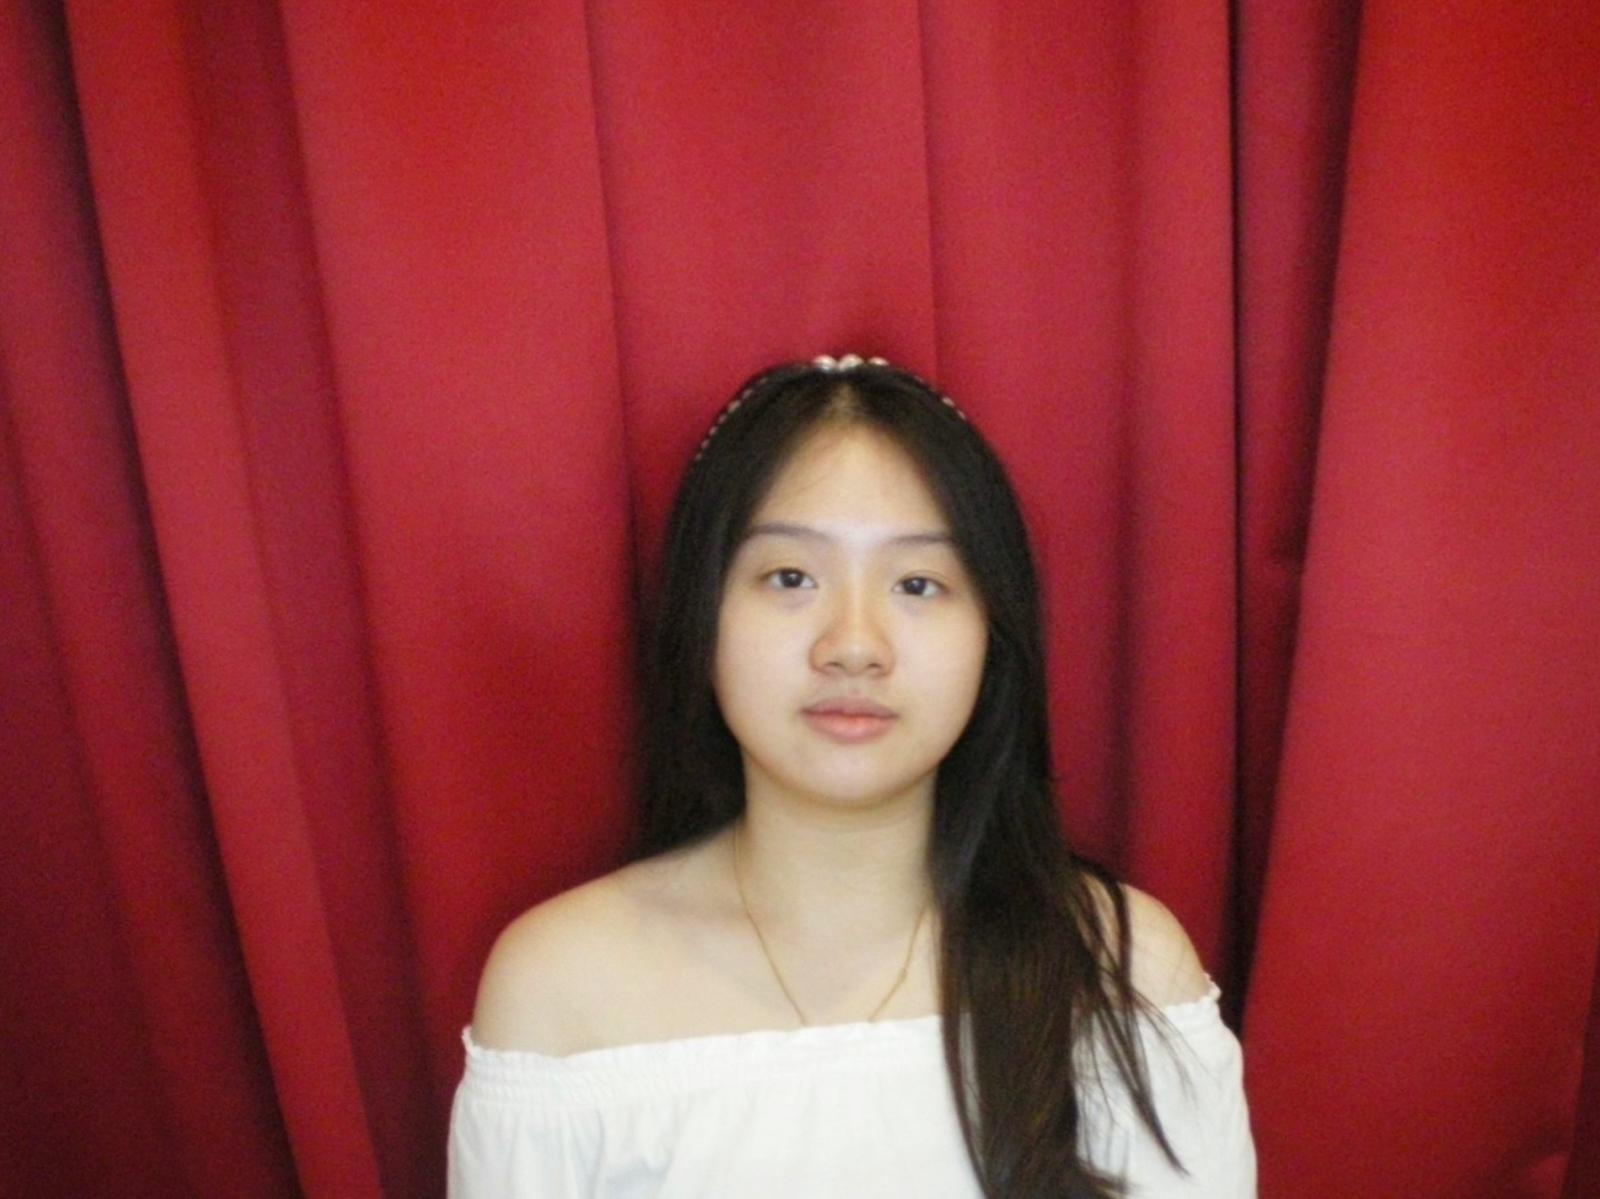
\includegraphics[width=\linewidth]{untitled.jpg} \\[34pt]	%trimming relative to image size

%---------------------------------------------------------------------------------------
%	META SKILLS
%----------------------------------------------------------------------------------------
\cvsection{SKILLS}

\cvskill{Python} {} {1} \\[-2pt]

\cvskill{Javascript} {} {0.9} \\[-2pt]

\cvskill{C\#} {} {0.7} \\[-2pt]

\cvskill{Java} {} {0.4} \\[-2pt]

\cvskill{Databases \& SQL} {Firebase, MSSQL} {0.9} \\[-2pt]

\cvskill{Back-end Development} {JavaScript, Node.js, Express.js} {0.85} \\[-2pt]

\cvskill{Front-end Development} {HTML, CSS, JavaScript, Bootstrap} {0.85} \\[-2pt]

\cvskill{User Experience Design} {Figma, Adobe} {0.8} \\[-2pt]

\cvskill{GIT} {} {0.7} \\[-2pt]




\vfill\null
\cvsection{CONTACT}
	
\icontext{MapMarker}{12}{30 Woodlands Dr 16, Forestville 11\#22\\Singapore 737769}{black}\\[6pt]
\icontext{MobilePhone}{12}{+65 98881351}{black}\\[6pt]
\begin{minipage}{\textwidth}
	\iconemail{Envelope}{12}{lawmingqi1818@gmail.com}{}{black}\\
	School: S10257808@connect.np.edu.sg
\end{minipage}\\[6pt]
	
\vfill\null

%---------------------------------------------------------------------------------------
%	EDUCATION
%----------------------------------------------------------------------------------------
\newpage
\cvsection{EDUCATION}

\cvmetaevent
{2019 - 2022}
{GCE 'O'Level Certificate}
{Orchid Park Secondary School}
{Achieved 6 distinctions in\\ E Maths, A Maths, Chinese,\\Science (Bio/Chem), \\Principles of Accounts,\\ Humanities (Social Studies/ History)  \\

L1R4: 11

L1R5: 13

}

\cvmetaevent
{Apr 2023 - Present}
{Diploma in Information \\
Technology}
{Ngee Ann Polytechnic}
{}

\vfill\null

%---------------------------------------------------------------------------------------
%	CERTIFICATION
%----------------------------------------------------------------------------------------
\newpage
\cvsection{CERTIFICATIONS}

\cvmetaevent
{PSM 1 - Professional Scrum Master 1}
{}
{}
{Certificate issued by Scrum.org to prove abilities in the fundamental level of Scrum mastery, including concepts of applying Scrum}

\cvmetaevent
{Google Project Management}
{}
{\cvlist{
	\item Project Execution: Running the Project
	\item Foundations of Project Management
	\item Project Planning: Putting It All Together
	\item Agile Project Management
	\item Project Initiation: Starting a Successful Project
}}
{Intense course designed to equip learners with in-demand project management skills.}


\cvmetaevent
{Online Tutorials}
{}
{}
{I believe in continuously expanding my knowledge beyond the classroom by exploring topics through online resources. I regularly take tutorials on platforms like LinkedIn and YouTube to reinforce what I’ve learned in class and to dive deeper into concepts.}
\vfill

\newpage
\mbox{} % hotfix to place qrcode on the bottom when there are not other elements
\vfill

\end{leftcolumn}
\begin{rightcolumn}
%---------------------------------------------------------------------------------------
%	TITLE  HEADER
%----------------------------------------------------------------------------------------
\fcolorbox{white}{royalpurple}{\begin{minipage}[c][3.5cm][c]{1\mpwidth}
	\begin {center}
		\HUGE{ \textbf{ \textcolor{white}{ \uppercase{ Law Ming Qi } } } } \\[-24pt]
		\textcolor{white}{ \rule{0.1\textwidth}{1.25pt} } \\[4pt]
		\large{ \textcolor{white} {Information Technology Student} }
	\end {center}
\end{minipage}} \\[-25pt]
\vspace{-12pt}

%---------------------------------------------------------------------------------------
%	PROFILE
%----------------------------------------------------------------------------------------
\vfill\null
\cvsection{PROFILE}

\cvtext{Proactive and goal-oriented IT student promoting well-developed skills in backend and frontend development and database management. Engaging demeanor known for working well in deadline-driven environments. \\

Driven by a passion for emerging technologies like quantum computing and DevOps, eager to explore these fields while strengthening core technical skills. Committed to continuous learning and growth in IT, with a focus on building scalable and maintainable solutions.\\

Adaptable and dedicated, with experience contributing effectively to diverse IT projects. Strong collaborator, ready to apply academic and industry knowledge to real-world challenges and looking to leverage acquired skills in a business setting.\\

} 

%---------------------------------------------------------------------------------------
%	WORK EXPERIENCE
%----------------------------------------------------------------------------------------
\vfill\null
\cvsection{WORK EXPERIENCE}

\cvevent
    {Aug 2023 - Oct 2023}
    {Retail and E-commerce Associate}
    {Cold Storage - Singapore}
	{}
    {\cvlist{
        \item Managed Online Orders: Processed and fulfilled online orders via Food Panda, ensuring timely and accurate delivery of grocery items.
        \item Grocery Selection and Replenishment: Picked and packed groceries efficiently, replenished stock, and ensured shelves were well-stocked to meet customer demand.
        \item Customer Assistance: Assisted customers in finding products, providing exceptional service, and addressing inquiries promptly to enhance the shopping experience.
    }}
	{}
	{}

\cvevent
	{Dec 2022 - Jan 2023}
	{Retail Assistant}
	{NTUC - Singapore}
	{}
	{\cvlist{
		\item Actively engaged with customers, providing general assistance and information on store merchandise to enhance the shopping experience.
		\item Replenished stock on the sales floor and maintained organized shelves, racks to ensure an attractive and easy-to-navigate store layout.
		\item Greeted customers, helped locate merchandise, and suggested suitable options.
	}}
	{}
	{}

\vfill\null

%---------------------------------------------------------------------------------------
%	AWARDS 
%----------------------------------------------------------------------------------------
\vfill\null
\cvsection{AWARDS}

\cvaward{2019}{
	Edusave Scholarship Award from Ministry of Education (MOE)}

\cvaward{2022}{
    Edusave Scholarship Award from MOE \\
    Edusave Award for Achievement, Good Leadership and Service \\
    Edusave Character Award
}


\vfill\null

%---------------------------------------------------------------------------------------
%	CO-CURRICULAR ACTIVITIES 
%----------------------------------------------------------------------------------------
\vfill\null
\cvsection{CO-CURRICULAR ACTIVITIES (CCA)}

\cvevent
	{2019 - 2022}
	{Orchid Park Secondary School}
	{Wushu}
	{\cvlist{
		\item \textbf{Captain}, Wushu School Team (2021 - 2022) – Led team training and provided coaching support.
		\item Participated in the \textbf{National School Games (NSG)} in 2021 and 2022.
		\item Achieved \textbf{Top 10} in the 2022 NSG for 1st International Nandao Female \\category.
	}}
	{}
	{}
	{}

\cvevent
	{2023 - Present}
	{Ngee Ann Polytechnic}
	{Wushu}
	{\cvlist{
		\item \textbf{Vice-Captain}, Wushu School Team (2023 - 2024) \\ – Organize training sessions and led team for competition and performance preparations.
		\item Responsible for choreographing routines for \textbf{group events}.
		\item \textbf{2nd Place}, NTU Invitational Wushu Championship 2023.
		\item \textbf{1st Prize}, Youth Category Female, 1st International Nandao.
		\item \textbf{1st Prize}, Open Category Group Event Non-weapon.
		\item \textbf{Performances}: 2024 Duanwu Delight (Chinese Culture Performance), Ngee Ann Kongsi Cheque Presentation Ceremony 2024.
	}}
	{}
	{\\\textcolor{royalpurple}{\textbf{Special Interest Group }}}
	{\cvlist{
		\item \textbf{Overflow:} \\
		Participated in a 3-day Data Structures and Algorithms Bootcamp, focused on problem-solving using Python.
		\item \textbf{ICT Society:} \\
		Assisted in the 2024 Graduation Ceremony for School of ICT to ensure smooth execution of the event.
	}}
	{}

\vfill\null

%---------------------------------------------------------------------------------------
%	ACADEMIC PROJECTS / COMPETITION PROJECTS 
%----------------------------------------------------------------------------------------
\vfill\null
\cvsection{ACADEMIC PROJECTS / COMPETITION PROJECTS }

\projects
    {Competition: National AI Student Challenge 2024}
    {Track 2 Amazon Web Services (AWS)}
    {Feb 2024 - March 2024}
    { 
        \item Amazon SageMaker
        \item AWS Cloud Services
        \item Large language model (LLM) - LLaMA-2-7B-Chat 
    }
    {
        \\\\
		\textbf{LLM Fine-Tuning:} Experimented with and adjusted various hyperparameters such as epochs, learning rate, and batch size to optimize the performance of the model for specific tasks.\\[5pt]
        \textbf{AWS SageMaker:} Gained hands-on experience with AWS SageMaker Jumpstart for managing end-to-end machine learning workflows, including model training and deployment.\\[5pt]
        \textbf{Data Preparation and Augmentation:} Learned to prepare custom datasets to enhance model performance.\\[5pt]
    }
    {}

\projects
    {Module: Back-end Development}
    {Community Engagement Website}
    {May 2024 - Jul 2024}
    { 
        \item Front-end: HTML, CSS, Javascript, Bootstrap
        \item Database: Firebase, MSSQL
        \item Back-end: Node.js, Express.js
        \item Tools: Firebase Cloud Storage, RESTful APIs, CRUD operations
    }
    {Middleware implementation, Graceful error handling, Firebase integration, User authentication (JWT), Responsive web design, CRUD operations, Real-time updates, RESTful API design}
	{
        \item Developed a \textbf{community club website} for users to \textbf{register}, \textbf{log in}, \textbf{update profile}, \textbf{book facilities}, \textbf{register for events}, and \textbf{provide feedback}, enhancing engagement and accessibility for club members.
        \item Designed a \textbf{responsive}, \textbf{user-friendly front-end} that ensures seamless access across devices.
        \item Integrated \textbf{Firebase} for \textbf{profile picture management}. Uploaded images are stored as files in \textbf{Firebase Storage}, with each image accessible via a unique \textbf{URL}.
        \item Implemented \textbf{authentication and authorization} using \textbf{JWT} and data protection measures through a hashing function, \textbf{bcrypt}.
        \item Managed backend data with \textbf{MSSQL}, handling \textbf{event registration}, \textbf{user profiles}, and \textbf{real-time announcements}.
        \item Developed \textbf{staff functionalities} with a dedicated \textbf{login system}, enabling staff to \textbf{manage} and \textbf{update website features}. Non-staff users have no access to these rights. \\[10pt]
    }


\vfill\null


%---------------------------------------------------------------------------------------
%	ACTIVITIES
%----------------------------------------------------------------------------------------
\vfill\null
\cvsection{ACTIVITIES}

\activities
	{Internation Experience}
	{Overseas Immersion Programme to Shenzhen, China}
	{March 2024}
	{Participated in a 2 weeks long immersion program in Shenzhen, China, focusing on both industrial and cultural visits}
	{
        \item \textbf{Industry Visits:} Engaged with leading tech companies and startups in Shenzhen such as Tencent and Minieye Technology, gaining insights into cutting-edge technologies and industry trends.
        \item \textbf{Cultural Exchange:} Immersed in Chinese culture like Wushu and Calligraphy and interacted with the professionals and students there, developing cross-cultural communication skills.
        \item \textbf{Cultural Visits:} Explored historic sites like Gankeng Hakka Town, enriching my understanding of traditional architecture and local customs while deepening my connection to Shenzhen’s cultural heritage.}
    {
        \item \textbf{Global Perspective:} Enhanced understanding of international IT trends and global market dynamics and competitions.
        \item \textbf{Technical Knowledge:} Gained exposure to technologies in China to power a range of applications from intelligent assistants to immersive gaming experiences.
        \item \textbf{Cultural Competence:} Improved ability to work in diverse cultural settings and communicate across cultures.
    }

\vfill\null

% hotfixes to create fake-space to ensure the whole height is used
\mbox{}
\vfill
\mbox{}
\vfill
\mbox{}
\vfill
\mbox{}
\end{rightcolumn}
\end{paracol}
\end{document}

